\documentclass[a4paper,11pt,twoside]{article}
%\documentclass[a4paper,11pt,twoside,se]{article}

\usepackage{UmUStudentReport}
\usepackage{verbatim}   % Multi-line comments using \begin{comment}
\usepackage{courier}    % Nicer fonts are used. (not necessary)
\usepackage{pslatex}    % Also nicer fonts. (not necessary)
\usepackage[pdftex]{graphicx}   % allows including pdf figures
\usepackage{listings}
%\usepackage{lmodern}   % Optional fonts. (not necessary)
%\usepackage{tabularx}
%\usepackage{microtype} % Provides some typographic improvements over default settings
%\usepackage{placeins}  % For aligning images with \FloatBarrier
%\usepackage{booktabs}  % For nice-looking tables
%\usepackage{titlesec}  % More granular control of sections.

% DOCUMENT INFO
% =============
\department{Institution för Datavetenskap}
\coursename{DV2: Algorithms and Problemsolving 7.5 p}
\coursecode{DV169VT16}
\title{OU5 Automata}
\author{Lorenz Gerber ({\tt{dv15lgr@cs.umu.se}} {\tt{lozger03@student.umu.se}})}
\date{2016-03-28}
%\revisiondate{2016-01-18}
\instructor{Lena Kallin Westin / Erik Moström / Jonathan Westin}


% DOCUMENT SETTINGS
% =================
\bibliographystyle{plain}
%\bibliographystyle{ieee}
\pagestyle{fancy}
\raggedbottom
\setcounter{secnumdepth}{2}
\setcounter{tocdepth}{2}
%\graphicspath{{images/}}   %Path for images

\usepackage{float}
\floatstyle{ruled}
\newfloat{listing}{thp}{lop}
\floatname{listing}{Listing}



% DEFINES
% =======
%\newcommand{\mycommand}{<latex code>}

% DOCUMENT
% ========
\begin{document}
\lstset{language=C}
\maketitle
\thispagestyle{empty}
\newpage
\tableofcontents
\thispagestyle{empty}
\newpage

\clearpage
\pagenumbering{arabic}

\section{Introduction} 
The subject of this assignment was to design and implement \textit{Push Down
Automata} (PDA) as a general datatype and apply it to simulate a
specific PDA that can process input according to \textit{reverse
  polish notation} (RPN) rules.

The formal defintion of a PDA is a 6-tuple consisting of the \textit{set of
States}, the \textit{input alphabet}, the \textit{stack alphabet},
\textit{transition functions}, a \textit{start state} and a set of
\textit{accepted states} \cite[p. 113]{sipser2012}. Push down automata can either be deterministic or
non-deterministic. The most prominent feature that distinguishes
push-down automata from other finite automata is the stack which allows to store information and process it later. 

\textit{Reverse Polish Notation} or RPN is a way of writing aritmethic
expressions. Instead of the common `in-fix' notation where an operator
is written between the two operands, RPN uses `post-fix' notation with
the operator after the operands. This way of indicating arithmetic
expressions makes paranthesis to modify the precedence of operators
obsolete. RPN has been used readily in financial and scientific pocket
calculators \cite{rpn}.  

\subsection{Push Down Automata Implementation}
The lab assignment proposed to represent the PDA either as a table or
as a graph. It was further communicated that the implementation shall be
\textit{finite} and \textit{deterministic}. \textit{Finite} defines
that independent of the input, the PDA will always terminate. The
\textit{deterministic} property defines that there can be in each
\textit{machine state} maximum one viable \textit{transition} to be
taken.   

Here it was decided to implement the PDA as a table. Initially, this
was not based on any research but more a `stomach feeling'.  To keep
the implementation as generic as possible it was further decided to 
separate checking the expression from calculating it. 


\section{Program Structure}
The main program is used to create and configure the PDA. Hence the
whole RPN logic is defined in the main program by creating and
assigning states and transitions. Then the PDA is executed. On
success, the actual RPN calculation function is called.

\subsection{Datatypes}

\subsubsection{pda - Push Down Automaton}
A generic implementation of a push down automaton according to Sipser \cite[pp.112-125]{sipser2012}.
The datatype \textit{pda} is constructed from a struct. It contains a
table (from course datatypes \cite{datatypes}, constructed from
dynamic list) with \textit{states}, a stack (from course datatypes
\cite{datatypes}, \textit{stack\_1cell}). The \textit{states} table contains
the transitions. The PDA contains further the variables
\textit{currentState} (pointer to the currently active state),
\textit{possibleTransition} (pointer to the next possible transition),
\textit{input} (pointer to the current position in the input string), 
\textit{inputLeft} (int for how many input chars left to process),
\textit{bailout} (flag that is set stop processing) and
\textit{succeed} (marker that becomes true when the input was verified
and the automaton is in an accepted state).

The functions in the interface that the user accesses are \textit{create}
(returns a new), \textit{pda\_addState} (to configure the
pda with a new state) and \textit{pda\_execute} (to run the PDA). The
functions \textit{pda\_setStartState},
\textit{pda\_getPossibleTransition} and \textit{pda\_doTransition} are
called from within \textit{pda\_execute}. 


\subsubsection{Alphabets}
Generally speaking, the \textit{input} alphabet includes
\textit{numbers}, \textit{operators}, \textit{blanks} and
\textit{EOF}. The \textit{Stack alphabet} contains single digit
\textit{numbers} and the \textit{dollar symbol} to mark the first
position in the stack.   

The alphabets were implemented as functions. There are two different
types of such alphabet functions: The first kind was used to check
input and stack for matching letters. In case of a match, those
functions return \textit{true}, otherwise \textit{false}. The other
kind of functions were used to reproduce the letter to be pushed on the
stack. They return the \textit{ASCII} code of the letter to be pushed. This
also includes a function that reads the current input letter and  
returns it.

By separating \textit{recognition} of the input string from
\textit{calculating} the expression, it was achieved that the pda
could be kept to operate on single \textit{chars} instead of
\textit{strings} or multi digit \textit{integers}.  

\subsubsection{States}
The representation of \textit{states} and \textit{transitions} for
a table based PDA can be done in various ways and the distinction
between \textit{state} and \textit{transition} is less clear than in a
graph based model. Here two different ways were considered: States
constructed only as a container for transitions, without any reference
to the alphabet. This requires a more complex transition
datatype. Alternatively, \textit{states} implemented according to 
the \textit{example 2.14} in Sipser \cite[p. 114]{sipser2012}, represented by
triple nested table (or an aggregated array) whith multi-columns for
each letter in the \textit{input alphabet} and subgroups as the 
individual columns for each letter of the \textit{stack alphabet}. Implementing
a representation for this model could be done with a nested table, an
array, where the logic for accessing the different levels is
integrated in the code or by a tree structure. Such a representation has
the advantage that it is directly visible whether a transition for a
certain state is defined or not as it has a unique location in
the data structure. When choosing a representation with states as mere
containers for transitions, a control mechanism to prevent assignment
of duplicate transitions is needed. 

Here, it was chosen to implement states as containers for
transitions. A state has an numeric \textit{id} and a directed list
with potential transitions to proceed along. The state itself is a
\textit{struct}. The interface of the \textit{state} is in the current
version very sparse. It contains just the functions
\textit{state\_create} (returns a new state) and
\textit{state\_addTransition} (to add transitions to the state).  

\subsubsection{Transition}
A transition needs to `know' whether it matches the current
state, it needs to define how to modify the current state and a
reference to the new/next state. In the current implementation, the
transition is a \textit{struct} with function pointers for the
\textit{alphabet} functions. Further, the transition contains an \textit{int}
of the destination state, \textit{destInt} and a char
\textit{description}. Note that in the current implementation, the
transition does not need to know its source state, hence, it could be
reused as long as the destination state matches. However, after
implementing the datatypes, it was found that reusing transitions
causes problems with the memory free functions: It happend that a
transition was attempted to be removed multiple times causing memory
errors. Hence, in the current version, for simplicity, instead of
reusing, multiple identical transitions were created.
  
The interface of the transition contains merely one function of
interest for the user, \textit{transition\_create}. All further
functions are used internal to check and apply the transitions. This
includes three functions to check for epsilon condition in the
transitiona (\textit{transition\_checkReadEpsilon,
  transition\_checkPopEpsilon, transition\_checkPushEpsilon}) and three
functions that wrap the \textit{alphabet} functions for input, stack
and push condition. 

\subsubsection{RPN Function}
As mentioned earlier, it was chosen to separate verification of the
input by the PDA from the calculation. The calculation is done by the
function \textit{rpn\_calc}. This function assumes that the input
statement is a valid RPN expression, hence the input is not
validated and it should as such just be used in conjunction with the
PDA datatype.

Compared to the PDA, the stack of the RPN calculator can hold multi
digit integers. In fact, integers are written to the stack just after
all their digits read from the input. Composing of multi-digit numbers
is done by using an `assembly' register and mulitplication by 10 in
every `round'. Blanks are interpreted as number terminators. In
beginning of the input, after operators and after terminating a number
read, blanks are disregarded. This behaviour agrees with the
implemented rule set in the RPN PDA. 

The parsing of \textit{char} type operators into real aritmethic
operators was inspired by a \textit{Stack Overflow} blog post using a
lookup table \cite{lookup}.

\section{RPN Expression Checking}

\begin{figure}
 \centering
  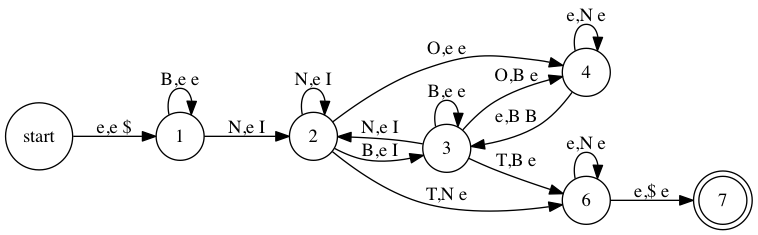
\includegraphics[width=\textwidth]{pda}
  \caption{\textit{Push Down Automata for Reverse Polish Notation. The small
    case `e' stands for `epsilon', the empty condition. `B' is a blank
  char, `N' any single-digit number char, `O' one of the four base
  arithmetic operators, `T' is EOF condition and the `\$' symbol is
  used as marker for an empty stack.}}
  \label{fig:rpn}
\end{figure}

The RPN logic is a use case of the generic PDA datatypes described
above. The automaton is represented as a graph in \textit{figure
  \ref{fig:rpn}}. It consists of seven states of which one
is the \textit{start state} \ref{tab:states}. \textit{State 6} is the
only \textit{accepting state}. There were a total of 15 transition
functions defined (\textit{table \ref{tab:trans}}). Each transition
consists of three letters: The condition for \textit{read},
\textit{pop} and the letter to be \textit{pushed} to the
stack. Further, for each transition, the destination state in case of
fulfilled \textit{read} and \textit{pop} criteria is indicated. The
\textit{stack-} and\textit{input alphabets} are shown in \textit{table
  \ref{tab:alphabet}}. Besides the letters in the alphabet, each of
the three positions in a transition statement can also be empty which
is usually shown by an lower case \textit{e} or $\epsilon$ (greek
epsilon). In the current implementation, epsilon is obtained by
\textit{NULL}.

\begin{table}[]
\centering
\caption{\textit{The states of the RPN Push Down Automaton}}
\label{tab:states}
\begin{tabular}{ll}
Id & Name                   \\
0  & start                  \\
1  & initialized            \\
2  & non-terminated         \\
3  & terminated             \\
4  & processing operand     \\
5  & check terminal         \\
6  & success               
\end{tabular}
\end{table}



\begin{table}[]
\centering
\caption{\textit{The table below shows the transitions used for the Reversed
  Polish Notation Push Down Automaton. The letter \textit{e} is used
  for \textit{epsilon}, \textit{B} as \textit{blank}, the letter
  \textit{I} for pushing \textit{input} to the stack. Further the
  letter \textit{O} and \textit{N} stand for \textit{operator} and
  \textit{number} respectively. \textit{T} stands for \textit{terminal} 
  and indicates the end of the input. The dollar sign is used as a
  letter of the stack alphabet to mark the first position. The column
  \textit{id} shows the id number of the transition in the C program.}}
\label{tab:trans}
\begin{tabular}{llllll}
id  & source & destination & read & pop & push \\ \hline
1   & start  & 1           & e    & e   & \$    \\
2   & 1      & 1           & B    & e   & e    \\
3\_1 & 1      & 2           & N    & e   & I    \\
3\_2 & 2      & 2           & N    & e   & I    \\
5   & 2      & 3           & B    & e   & I    \\
4   & 2      & 4           & O    & e   & e    \\
6   & 2      & 6           & T    & N   & e    \\
3\_3 & 3      & 2           & N    & e   & I    \\
13  & 3      & 3           & B    & e   & e    \\
7   & 3      & 4           & O    & B   & e    \\
8   & 3      & 6           & T    & B   & e    \\
9   & 4      & 4           & e    & N   & e    \\
10  & 4      & 5           & e    & B   & B    \\
11  & 6      & 6           & e    & N   & e    \\
12  & 6      & 7           & e    & \$   & e   
\end{tabular}
\end{table}

\begin{table}[]
\centering
\caption{\textit{Alphabets of the the RPN automaton}}
\label{tab:alphabets}
\begin{tabular}{ll}
alphabet & values                                   \\ \hline
input    & blank, number, operator, EOF \\
stack    & '\$', number                
\end{tabular}
\end{table}


\subsubsection{Problem Solving Strategy}
In the RPN automaton's first transition from \textit{start} to \textit{state
1}, a dollar symbol is pushed on the stack to mark it as
\textit{empty}. In the first state, the machine can read an arbitrary
number of blanks ($B,\epsilon \rightarrow \epsilon$).

The main logic is in \textit{states 2,3,4}. \textit{State 2} and
\textit{3}, `non-terminated' and `terminate' refer to reading an
operand from the input. It is considered `terminated' when a
number is followed by either an \textit{operator} or a
\textit{blank}. In the `terminated' state, either an \textit{operator}
or an \textit{EOF} is accepted. When an \textit{operator} is accepted
from the input, \textit{state 4} is accessed. Here, the last number
(single or multi-digit) is popped sequentially from the stack
($\epsilon,N \rightarrow \epsilon$). The other possible transition
requires to pop an blank from the stack ($\epsilon, B \rightarrow
B$). As blanks are just pushed between numbers, it guarantees that the
automaton just proceeds after an operator if there are at least two
numbers on the stack. The second operand is not popped from the stack
as it represents now the result of the arithmetic operation. Instead,
the number is `terminated' again with a blank.  

When the input string is used up, the automaton tranistions to
\textit{state 6}. This is possible either from `terminated' or
`non-terminated' state. When coming from the `terminated' state, the
blank is popped. To make sure that there is just the the result left
on the stack, from \textit{state 6} only numbers (or finally the
dollar symbol) can be popped. After popping the dollar symbol, the
automaton ends up in the only accepted state.

Hence, the processing stops when there is no more viable transition to
take. If the automaton is in a accepted state, the \textit{succeed}
flag is raised in the \textit{pda} datatype. 


\subsection{Testing}
A range of different inputs where tested. The testcases can be found
in \textit{table \ref{tab:test}}. Most interesting cases are related
to blanks either before, between or after numbers and operators. All
cases that could be thought of succeeded. Neither the \textit{pda} automaton
nor the \textit{rpn\_calc} function check for the size of
numbers. Hence it can happen that a result is too big for the datatype
\textit{int} and `goes around'.  

\begin{table}[]
\centering
\caption{\textit{Test cases for the RPN PDA}}
\label{tab:test}
\begin{tabular}{lll}
expression          & expected           & test \\ \hline
``''                  & Invalid expression & ok   \\
``1''                 & 10                 & ok   \\
``0''                 & 0                  & ok   \\
``01''                & 1                  & ok   \\
``1 1''               & Invalid expression & ok   \\
``a1''                & Invalid expression & ok   \\
``0 1/''              & 0                  & ok   \\
``   1 1  +  ''       & 2                  & ok   \\
``11111 11111*''      & 1234554321         & ok   \\
``111111 111111*''    & -539247567         & ok   \\
``10 20-''            & -10                & ok   \\
``1 2 + 3 - 4 * 5 /'' & 0                  & ok   \\
``1 2 3 +''           & Invalid expression & ok   \\
``*''                 & Invalid expression & ok  
\end{tabular}
\end{table}

\section{Extra Assignment - Bracket Matching}
After the basic datatypes and the RPN automaton were implemented, it
was investigated how flexible the program would be for another
automaton. For this, the \textit{Bracket Matching} automaton was
implemented. After copying the \textit{main} program of the RPN
automaton, adjusting took just a few minutes. Basically, three states
and five transitions had to be defined.  Addiontally, three new
\textit{alphabet} functions were written: \textit{isOpeningBracket},
\textit{isClosingBracket} and \textit{openingBracket}. Finally, the
RPN calculation function was removed from main. The program uses all
the same header files and is available in the file
\textit{bracket\_automat.c}. The input expressions given in the
lab description were tested and succeded.

\section{Discussion}
The chosen design is very flexible for implementing generic automata
as demonstrated with the \textit{Bracket Matching} automaton. The
chosen separation of datatypes works well and allows for quick
reconfiguration of the automaton. It can be argued whether the
\textit{State} datatype is needed at all. Instead, one could include
also the source state in the transitions. Also the information about
accepted / non-accepted state could be included in the
transition itself. This would however result in more redundant information
and the need for validating it to prevent inconsistent user input.

Admittedly, as mentioned in the description to the lab assignment, 
a grpah would probably have been a more natural basis for this
datatype. 

During the design and plannig phase, the largest concerns were about
conversions between \textit{char}'s and \textit{int}'s aswell as single
and multi-digit numbers on the stack. The \textit{PDA} is easiest to implement
when each stack register just holds one \textit{char}. This
corresponds also to the theoretical description of a
\textit{PDA}. However, for the calculation, multi-digit numbers have 
to be handled. It was tempting to implement multi-digit numbers on the
stack but it would possibly make the pda less generic. After various
rejected designs (including using separate \textit{registers} in the
\textit{PDA} for calculation), the author finally settled for a
puristic \textit{PDA} implementation with a separated calculation
function. The \textit{PDA} works so to say as input validator which
allows to keep the \textit{RPN} calculator very simplistic as no input
validation needs to be done.  


\addcontentsline{toc}{section}{\refname}
\bibliography{references}

\end{document}
